\subsection{Økologisme}
For at forstå, hvilket budskab, spillet skal bringe, bliver vi nødt til at forstå økologismen. Ifølge Britannica, er økologisme en politiske bevægelse, der ønsker at forbedre eller beskytte naturen, det vilde, der opleves som intrinsisk godt. Dette skal opnås ved at begrænse menneskelig adfærd, der opfattes som skadelig overfor naturen. Biprodukter ved menneskelig adfærd som udledningen af eksempelvis skrald i naturen opfattes som negative eksternaliteter, der korumperer det her intrinsiske gode i naturen. Især også menneskeforårsaget udledning af kuldioxid- og andre drivhusgasser er ifølge økologi-bevægelsen en af de store syndere i klimaregneskabet.

Begrænsningen skal bl.a. opnås ved hjælp af politisk handling og lovgivning.\footfullcite{environmentalism_britannica}

Økologismen blev især stor i 2019, da Greta Thunberg holdte sin da den dengang 16-årige Greta Thunberg holdte sin ``You have stolen my dreams and my childhood'' og ``How dare you''-tale. Her anklagede hun ældre generationer for ikke at have gjort nok.\footfullcite{gretathunberg}

\subsection{Målgruppefastsættelse}
Produktet er målrettet til jævnaldrende Gen Z'ere (født mellem 1997 og 2012), idet det vurderes, at økologismen i stor grad kan appellere til denne målgruppe, hvorfor vores resurser ikke vil være spildt på dem. Desuden er gruppen også en praktisk størrelse, idet vi omgås dem, hvorfor vi bedre kan interagere og lade dem interagere med vores produkt

\subsection{Om plastikophobning}
Plastik forurening udgør i havene et stadigt voksende problem. Store mængder af plastikaffald bliver udledt i havet hvert år og samles i havstrømmene, hvor de danner ``garbage patches''\footfullcite{natgeo2025}. 

Den mest kendte og den absolut største af disse ophobninger er \textit{The Great Pacific Garbage Patch}, som befinder sig i det nordlige Stillehav. Forskning viser, at \textit{The Great Garbage Patch} indeholder omkring 1,8 billioner stykker plastik (dvs. 1.800 miliarder) spredt over et område på omkring 1,6 millioner kvadratkilometer\footfullcite{oceancleanup2026}. Det er svært at forestille sig, hvor stort det er. Men til sammenligning er hele Danmarks areal er lidt over 43.000 kvadratkilometer, så det svarer til at have mere end 37 Danmark i størrelse fyldt med plastikaffald.

\begin{figure}[H]
    \centering
    \fbox{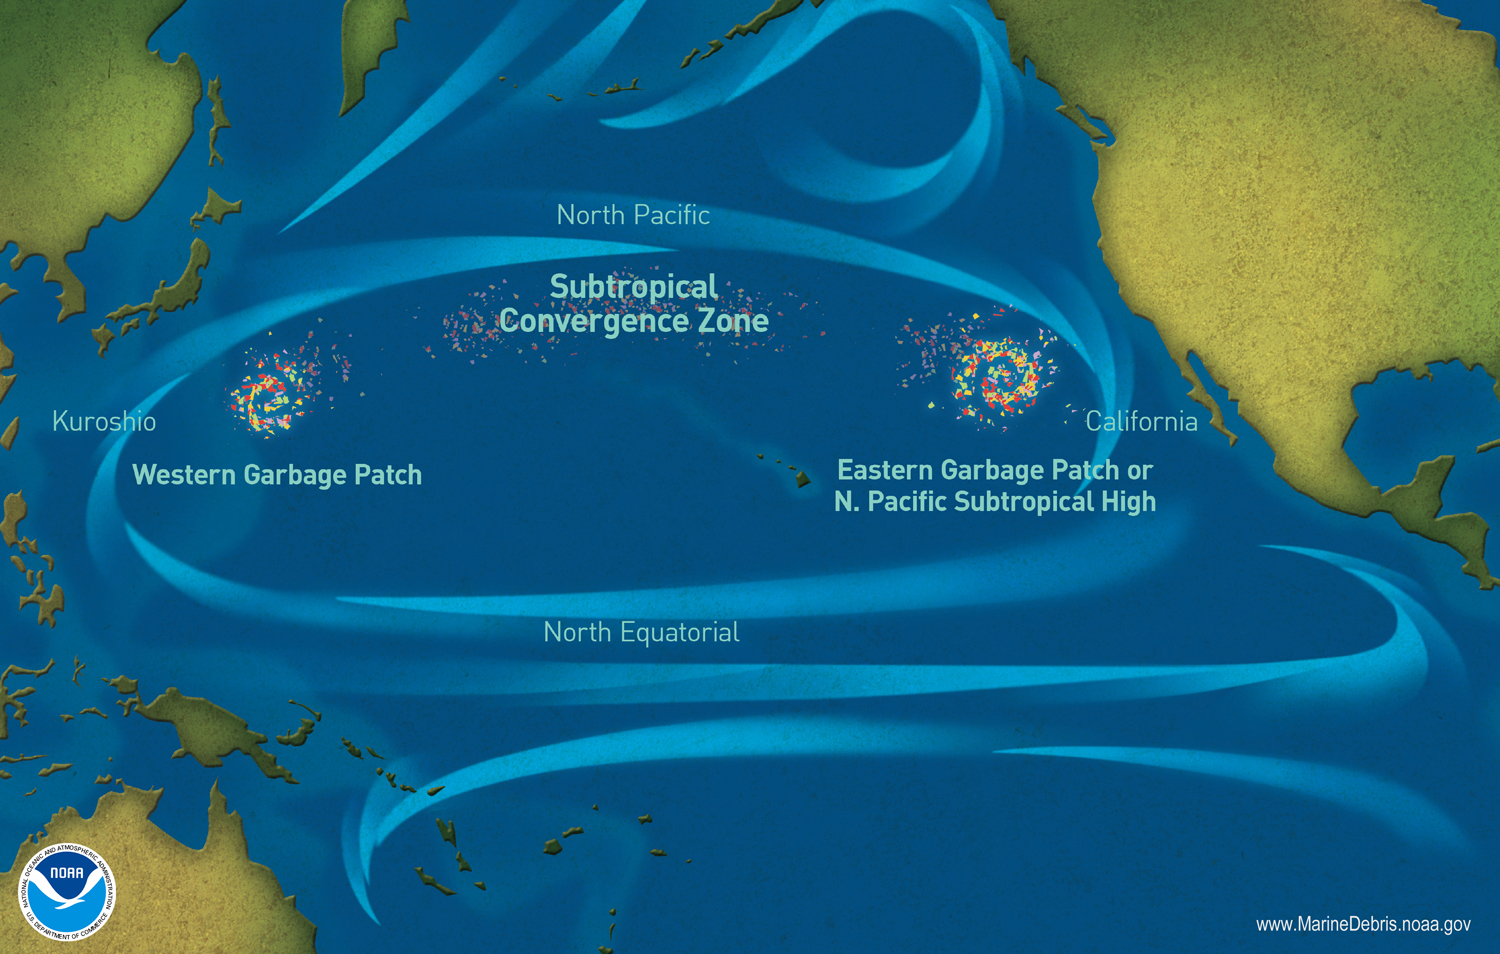
\includegraphics[width=0.6\textwidth]{assets/great-pacific-garbage-patch.jpg}}
    \caption{The Great Pacific Garbage Patch\cite{oceancleanup2026}}\label{fig:oceanstreams}
\end{figure}

Plastiophobningerne skyldes, at når plastikaffald ender i havet, bliver det transporteret af havstrømmene og samles i spcifikke områder i havet, hvor strømmene mødes og skaber cirkulære bevægelser. Disse strømme kan ses på \autoref{fig:oceanstreams} som viser \textit{The North Pacific Gyre}.

Plastik i havet udgør en meget alvorlig trussel mod havets økosystemer og dyreliv. Mange dyr i havet forveksler plastik med og spiser det fejlagtigt, hvilket fører til hæftige skader på deres fordøjelsessystemer og i værste fald død. Plastik nedbrydes ikke let i naturen og nedbrydes i stedet til mindre og mindre stykker, der kan være endnu mere skadelige for dyrelivet, og det gør det også nært umuligt at fjerne fra havet igen.

Den palstik som bliver nedbrudt til mindre dele, og ender i fiskene, har en direkte effekt på mennesker, da vi spiser fiskene får vi det mikroplastik ind i vores krop.

Steam er en digital platform som distribuerer spil til millioner af brugere verden over.

Steam udgiver, hver måned en undersøgelse som deres brugere frivilligt kan deltage i. Undersøgelsen omhandler hvilken hardware og software deres brugere har. Disse tal er utroligt vigtige for os, da det giver os en indikation af, hvilken hardware vores spil skal kunne køre på.\footfullcite{steamSurvey2026}

Vi noterer os, at 51,93\% af Steam brugere har en skærmopløsning på 1920x1080 og udgør derfor normen for skærmopløsning, selvom tendensen er skiftende. Det er således også det, vi tager udgangspunkt i, når vi laver størrelserne på ting i vores spil.
